\documentclass{beamer}
\usetheme{me} % aalto theme


% Packages for math, language, encoding etc.
\usepackage{tikz, ctable}
\usepackage{bm}
\usepackage[english]{babel}
\usepackage[utf8]{inputenc}
\usepackage{graphicx}
\usepackage{xcolor}
\usepackage[absolute,overlay]{textpos}	
\usepackage{amsfonts,amssymb,amsbsy,amsthm,amsmath,mathtools,enumerate,verbatim}
\usepackage{stmaryrd} % double square brackets
\usepackage{color, colortbl}
\usepackage[font=scriptsize]{caption}
\usepackage{csquotes}
\usepackage{tabularray}
\usepackage{hyperref}
\usepackage{datetime}
\usepackage{pifont}

% For def of elliptical distributions

% Bibliography and style.
\usepackage[style=authoryear, maxcitenames=2]{biblatex}
\addbibresource{sources.bib}
\setbeamertemplate{bibliography item}{}

%\usepackage[
%  backend=biber,
%  style=authoryear,
%]{biblatex}
%\addbibresource{sources.bib}

% Show greyed table of contents before section.
\AtBeginSection[]
{
    \begin{frame}
        \frametitle{Table of Contents}
        \tableofcontents[currentsection]
    \end{frame}
}
\setcounter{tocdepth}{1}


\AtBeginSubsection[]{
  \begin{frame}
  \vfill
  \centering
  \begin{beamercolorbox}[sep=8pt,center,shadow=true,rounded=true]{subtitle}
    \usebeamerfont{subtitle}\insertsubsectionhead\par%
  \end{beamercolorbox}
  \vfill
  \end{frame}
}

% Info about presentation
\title{Moment Estimator-Based Extreme Quantile Estimation with Erroneous Observations}
\subtitle{Joint work with Pauliina Ilmonen and Lauri Viitasaari \\
\url{https://doi.org/10.48550/arXiv.2502.08510}}
\author{Jaakko Pere}

\newdate{date}{28}{5}{2026}
\date{\displaydate{date}}

% Own commands and math operators.
%\newcommand{\xRightarrow}[2][]{\ext@arrow 0359\Rightarrowfill@{#1}{#2}}
\newcommand{\R}{\mathbb{R}} % Real numbers
\DeclareMathOperator{\rank}{rank}
\DeclareMathOperator{\var}{Var}
\DeclareMathOperator{\trace}{trace}
\newcommand{\Rg}{\mathcal{R}}
\newcommand{\U}{\mathcal{U}}
\newcommand{\D}{\mathcal{D}}
\newcommand{\Sp}{\mathbb{S}}
\newcommand{\tens}[1]{%
  \mathbin{\mathop{\otimes}\displaylimits_{#1}}%
}
\DeclareMathOperator{\mda}{MDA}
\DeclareMathOperator{\rv}{RV}
\DeclareMathOperator{\erv}{ERV}
% Page number
%\setbeamertemplate{footline}[frame number]

%%%%%%%%%%%%%%%%%%%%%%%%%%%%%%%%%%%%%%%%%%%%%%%%%%%%%%%%%%%%%%%%%%%%%%%%%%%%%%%
%%%%%%%%%%%%%%%%%%%%%%%%%%%%%%% DOCUMENT BEGINS %%%%%%%%%%%%%%%%%%%%%%%%%%%%%%%
%%%%%%%%%%%%%%%%%%%%%%%%%%%%%%%%%%%%%%%%%%%%%%%%%%%%%%%%%%%%%%%%%%%%%%%%%%%%%%%
\begin{document}

\frame{\titlepage}

\begin{frame}{Agenda of the Presentation}
\tableofcontents
\end{frame}

%%%%%%%%%%%%%%%%%%%%%%%%%%%%%%%%%%%

\section{Motivation}

%%%%%%%%%%%%%%%%%%%%%%%%%%%%%%%%%%%

\begin{frame}{Extreme Value Theory: Tools for Extrapolation}
  \begin{itemize}
    \item Extreme value theory is concerned with inference of rare events.
    \pause
    \item Consider estimating $0.999$-quantile (red cross) with a reasonable
    sample (black circles). 
  \end{itemize}
  \pause
  \begin{figure}
    \centering
    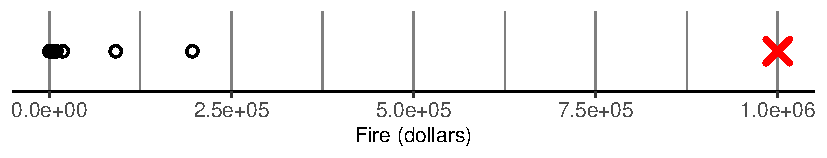
\includegraphics[width = \textwidth]{figures/fire-quantile-crop}
    \caption{Insurance company keeps records of fire insurance claims per
    windstorm. In total, the figure shows 700 observations.}
  \end{figure}
\end{frame}

%%%%%%%%%%%%%%%%%%%%%%%%%%%%%%%%%%%

\begin{frame}{Noisy Observations}
  What if instead of the original observations only approximations are
  available?
  \begin{itemize}
    % Real life data is always discrete (only finite number of digits can be
    % stored)
    \item[$\Rightarrow$] Extreme value inference with the noisy sample.
  \end{itemize}
  \pause
  Why?
  \pause
  \begin{itemize}
    % Data is always discrete (only finite number of digits can be stored
    % Only approxximations available (always the case with functional data)
    \item Extreme value index estimation for projections of functional
    data~\parencite{kokoszka2018}.
    \item Extreme quantile/expectile regression~\parencite{girard2021}.
    \item Latent model extreme value index estimation~\parencite{virta2024}.
  \end{itemize}
  \pause
  Much more work has been done especially in the heavy-tailed case (few or no
  moments exist)...
\end{frame}

%%%%%%%%%%%%%%%%%%%%%%%%%%%%%%%%%%%

\begin{frame}{Approaches from the Literature (for the Heavy Tail)}
  1. \parencite{kim2020, kim2023b}: We have $\hat Y_i = Y_i + \varepsilon_i$, where
  \begin{itemize}
    \item the errors $\varepsilon_i$ are i.i.d.,
    \item $\{Y_i\} \perp\kern-5pt \perp\{\varepsilon_i\}$, and
    \item $\lim_{t\to\infty}\mathbb{P}(|\varepsilon| > t)/\mathbb{P}(X_1 > t) = 0$
  \end{itemize}
  \pause
  \textcolor{orange}{2. \parencite{girard2021}: We have that the errors $|\hat
  Y_i - Y_i|$}
  \begin{itemize}
    \item can be dependent,
    \item they do not need to be identically, distributed, and
    \item $\{Y_i\} \perp\kern-5pt \perp\{\varepsilon_i\}$ can fail.
    \item $\max_{i\in\{1\ldots, n\}}|\hat Y_i -
    Y_i|/Z_n\stackrel{\mathbb{P}}{\to} 0$, as $n\to\infty$.
    \end{itemize}
\end{frame}

%%%%%%%%%%%%%%%%%%%%%%%%%%%%%%%%%%%

\begin{frame}{Scope of the Presentation}
  1. We quantify the effect of approximation errors for a certain \emph{extreme
  quantile estimator}:
  \begin{itemize}
    \item Short-, light-, and heavy-tailed distributions are considered. 
  \end{itemize}
  \pause
  2. Application to multivariate extreme quantile region estimation under
  ellipticity.
\end{frame}

%%%%%%%%%%%%%%%%%%%%%%%%%%%%%%%%%%%

\section{Preliminaries of Extreme Value Theory}

%%%%%%%%%%%%%%%%%%%%%%%%%%%%%%%%%%%

\begin{frame}{Maximum Domain of Attraction ($Y\in \mda\left(G\right)$)}
  Let $Y_1, \ldots, Y_n$ be i.i.d.\ observations of a random variable $Y$. We
  have $Y\in\mda\left(G\right)$ if there exist sequences $a_n > 0$ and
  $b_n\in\mathbb{R}$, and a random variable $G$ with a nondegenerate
  distribution such that
\begin{equation*}
	\frac{\max\left(Y_1, \ldots, Y_n\right) - b_n}{a_n}
  \stackrel{\mathcal{D}}{\to} G, \quad n\to\infty.
\end{equation*}
\end{frame}

%%%%%%%%%%%%%%%%%%%%%%%%%%%%%%%%%%%

\begin{frame}{Extreme Value Index \parencite{fisher1928,gnedenko1943}}
  Up to location and scale, the distribution of $G = G_\gamma$ is characterized
  by the parameter $\gamma$, called the \emph{extreme value index}. That is, the
  distribution of ${G_\gamma}$ is of the type
  \begin{equation*}
    F_{G_\gamma}\left(x\right) =
    \begin{cases}
      \exp\left(-\left(1 + \gamma x\right)^{-1/\gamma}\right),
      \quad 1 + \gamma x > 0 &\textnormal{if}\quad \gamma\neq 0, \\
      \exp\left(-e^{-x}\right),
      \quad x\in\mathbb{R} &\textnormal{if}\quad \gamma = 0.
    \end{cases}
  \end{equation*}
\end{frame}

%%%%%%%%%%%%%%%%%%%%%%%%%%%%%%%%%%%

\begin{frame}
  Maximum domain of attraction $\mda\left(G_\gamma\right)$ for different values
  of the extreme value index $\gamma$.
  \begin{table}
    \small
    \centering
    \begin{tabular}{c|c|c}
      $\gamma$ & Example of $F\in\mda\left(G_\gamma\right)$ & Properties of $F$
      \\
      \hline\hline
      $> 0$ & Pareto distribution & For a larger $\gamma$ fewer moments exist*
      \\
      $= 0$ & Normal distribution & All moments exist* \\
      $< 0$ & Uniform distribution & Finite endpoint
    \end{tabular}
  \end{table}
  *The claims about the moments hold if the left tail of a distribution is not
  considered.
\end{frame}

%%%%%%%%%%%%%%%%%%%%%%%%%%%%%%%%%%%

\begin{frame}{Tail Quantile Function}
  Define the tail quantile function corresponding to a distribution $F$ by
  \begin{equation*}
    U\left(t\right) = F^{\leftarrow}\left(1 - \frac{1}{t}\right), \quad t > 1,
  \end{equation*}
  where we denote the left-continuous inverse of a nondecreasing function by
  $f^\leftarrow\left(y\right) = \inf\left\{x\in\mathbb{R} : f(x) \geq
  y\right\}$.
  \vspace*{0.5cm}
  \pause

  That is, $U\left(1/p\right)$ is the $(1-p)$-quantile.
\end{frame}

%%%%%%%%%%%%%%%%%%%%%%%%%%%%%%%%%%%

\begin{frame}{MDA Condition in Terms of Quantiles \parencite{dehaan1984}}
  
  Let $U$ be the tail quantile function corresponding to a random variable $Y$.
  Then, $Y\in\mda\left(G_\gamma\right)$ if and only if there exists a positive
  function $a:\mathbb{R}^+ \to \mathbb{R}^+$ such that for all $x > 0$,
  \begin{equation*}
    \lim_{t\to\infty}\frac{U\left(tx\right) - U\left(t\right)}
    {a\left(t\right)} = \frac{x^\gamma - 1}{\gamma}.
    % For $\gamma = 0$ RHS interpreted as $\ln x$.
  \end{equation*}
  \pause
  Choose $t=n/k$ and $x = k/(np)$ to get the approximation
    \begin{equation*}
      U\left(\frac{1}{p}\right)\approx U\left(\frac{n}{k}\right) +
      a\left(\frac{n}{k}\right)
      \frac{\left(\frac{k}{np}\right)^{\gamma} - 1}{\gamma}.
    \end{equation*}
\end{frame}

%%%%%%%%%%%%%%%%%%%%%%%%%%%%%%%%%%%

\begin{frame}{Extreme Quantile Estimation}
  Suppose $\bm Y = \left(Y_1, \ldots, Y_n\right)$ is an i.i.d.\ sample of
  $Y\in\mda\left(G_\gamma\right)$, $\gamma\in\mathbb{R}$. Denote order
  statistics corresponding to the sample $\bm Y$ by $\bm Y_{1, n} \leq \dots
  \leq \bm Y_{n, n}$. Then an estimator for the extreme $(1-p)$-quantile $x_{p}
  = U\left(1/p\right)$ can be given as
  \begin{equation*}
    \hat x_{p}\left(\bm Y\right) = \bm Y_{n-k,n} +
    \hat{a}\left(\frac{n}{k}\right)
    \frac{\left(\frac{k}{np}\right)^{\hat\gamma\left(\bm Y\right)} - 1}
    {\hat\gamma\left(\bm Y\right)},
  \end{equation*}
  where $\hat\gamma$ is an estimator for the extreme value index $\gamma$.
\end{frame}

%%%%%%%%%%%%%%%%%%%%%%%%%%%%%%%%%%%

\begin{frame}{The Moment Estimator \parencite{dekkers1989}}
  Set, for  $\ell\in\{1, 2\}$,
  \begin{equation*}
    M_n^{(\ell)}\left(\bm Y\right) = \frac{1}{k}\sum_{j=0}^{k-1}
    \left(\ln \bm Y_{n-j, n} - \ln \bm Y_{n-k, n}\right)^\ell,
  \end{equation*}
  and
  \begin{equation*}
    \hat\gamma_+\left(\bm Y\right) = M_n^{(1)}\left(\bm Y\right)
    \quad\textnormal{and}\quad
    \hat\gamma_-\left(\bm Y\right) = 1
    - \frac{1}{2}\left(1 - \frac{\left(M_n^{(1)}\left(\bm Y\right)\right)^2}
    {M_n^{(2)}\left(\bm Y\right)}\right)^{-1}.
  \end{equation*}
  Then the moment estimator is defined as
  \begin{equation*}
    \textcolor{orange}{\hat\gamma_M\left(\bm Y\right)
    = \hat\gamma_+\left(\bm Y\right)
    + \hat\gamma_-\left(\bm Y\right)},
  \end{equation*}
  and the corresponding estimator for $a\left(n/k\right)$ is defined as
  \begin{equation*}
    \textcolor{orange}{
    \hat\sigma_M\left(\bm Y\right) = \bm Y_{n-k, n} M_n^{(1)}
    \left(\bm Y\right)\left(1 - \hat\gamma_-
    \left(\bm Y\right)\right)}.
  \end{equation*}
\end{frame}

%%%%%%%%%%%%%%%%%%%%%%%%%%%%%%%%%%%

\section{Extreme Value Theory with Approximations}

%%%%%%%%%%%%%%%%%%%%%%%%%%%%%%%%%%%

\begin{frame}{Back to Approximations}
  \begin{itemize}
    \item What if instead of the sample $\bm Y$, only approximations $\hat{\bm Y}
    = (\hat Y_1, \ldots, \hat Y_n)$ are available?
    \pause
    \item How the approximation error affects the asymptotics?
  \end{itemize}
  \vspace*{0.5cm}
  \pause

  That is, next we quantify how the error
  \begin{equation*}
    \max_{0\leq j\leq k} \left|\frac{\hat{\bm Y}_{n-j,n}}{\bm Y_{n-j,n}}
    - 1\right|
  \end{equation*}
  has to behave in order to have asymptotic normality for $\hat x_p(\hat{\bm
	Y})$.
\end{frame}

%%%%%%%%%%%%%%%%%%%%%%%%%%%%%%%%%%%

\begin{frame}{Assumptions for the Main Result}
  \begin{enumerate}
    \item $Y$ is an almost surely positive random variable with $F\in
	  \mathcal{D}\left(G_\gamma\right)$, $\gamma\in\mathbb{R}$ (and $U$ satisfies
	  certain second-order conditions).
    \item $\bm Y = \left(Y_1, \ldots, Y_n\right)$ are i.i.d.\ copies of $Y$ and
	  let $\hat{\bm Y} = (\hat Y_1, \ldots, \hat Y_n)$ be an approximated sample.
    \pause
    \item Suppose $k = k_n\to\infty, k_n/n\to 0$, as $n\to\infty$.
    \item $p = p_n$, $np_n = o\left(k_n\right)$ and $\ln\left(np_n\right) =
		o\left(\sqrt{k_n}\right)$.
  \end{enumerate}
\end{frame}

%%%%%%%%%%%%%%%%%%%%%%%%%%%%%%%%%%%

\begin{frame}{Sketch of the Main Result}
	Suppose that assumptions of the previous slide hold and that
	\begin{equation*}
		\max_{0\leq j\leq k_n} \left|\frac{\hat{\bm Y}_{n-j,n}}
		{\bm Y_{n-j,n}} - 1\right|
		= O_\mathbb{P}\left(h_n\right)
	\end{equation*}
	for some sequence $h_n$ such that  $\textcolor{orange}{\sqrt{k_n}
	\frac{h_nU\left(\frac{n}{k_n}\right)}{a\left(\frac{n}{k_n}\right)} = o(1)}$.
	Denote $q_\gamma\left(t\right) = \int_1^t s^{\gamma - 1}\ln s \, \mathrm{d}s$.
	Then
  \begin{equation*}
    \sqrt{k_n}\frac{\hat x_{p_n}(\hat{\bm Y})
		- U\left(1/p_n\right)}{a\left(\frac{n}{k_n}\right)
		q_\gamma\left(\frac{k_n}{np_n}\right)}
  \end{equation*}
  is asymptotically normal.
\end{frame}

%%%%%%%%%%%%%%%%%%%%%%%%%%%%%%%%%%%

\begin{frame}{Condition for the Error}
  Suppose $k = k_n\to\infty, k_n/n\to 0$, as $n\to\infty$. Assume also that $U$
  satisfies a certain second-order condition and that
  \begin{equation*}
		\max_{0\leq j\leq k_n} \left|\frac{\hat{\bm Y}_{n-j,n}}
		{\bm Y_{n-j,n}} - 1\right|
		= O_\mathbb{P}\left(h_n\right)
	\end{equation*}
	for some sequence $h_n$. Then $\textcolor{orange}{\sqrt{k_n}
	\frac{h_nU\left(\frac{n}{k_n}\right)}{a\left(\frac{n}{k_n}\right)}\to 0}$ if
  \begin{enumerate}
		\item $\gamma > 0$ and $\sqrt{k_n} h_n \to 0$,
		
		\item $\gamma = 0$ and $\sqrt{k_n} h_n =
		O\left(\left(\frac{n}{k_n}\right)^{-\delta}\right)$ for some $\delta > 0$,

		\item $\gamma < 0$ and $\sqrt{k_n} h_n =
		o\left(\left(\frac{n}{k_n}\right)^{\gamma}\right)$.
	\end{enumerate}
\end{frame}

\begin{frame}{Example}
  If
  \begin{equation*}
		\max_{0\leq j\leq k_n} \left|\frac{\hat{\bm Y}_{n-j,n}}
		{\bm Y_{n-j,n}} - 1\right|
		= O_\mathbb{P}\left(\frac{1}{\sqrt{n}}\right),
	\end{equation*}
  then the sufficient condition for the error does not hold if $\gamma\leq
  -1/2$!
\end{frame}

\section{Extreme Quantile Region Estimation under Ellipticity}

%%%%%%%%%%%%%%%%%%%%%%%%%%%%%%%%%%%

\begin{frame}
  \begin{center}
    \begin{figure}
      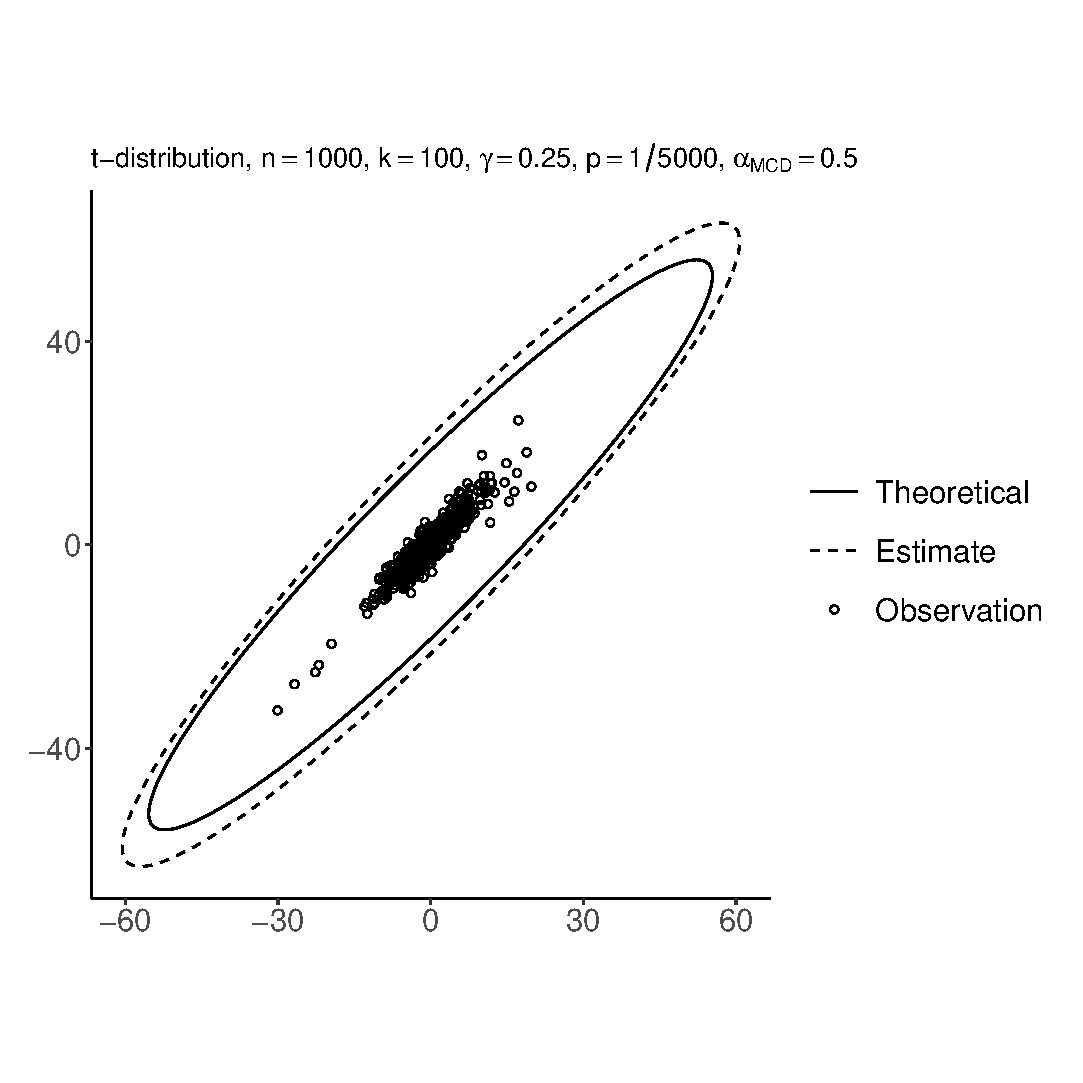
\includegraphics[width=0.8\textwidth, height=0.8\textwidth]{figures/idea}
    \end{figure}
  \end{center}
\end{frame}

%%%%%%%%%%%%%%%%%%%%%%%%%%%%%%%%%%%

\begin{frame}{Extreme Quantile Region Estimation}
  Let $X\in\mathbb{R}^d$ be a random vector with density $f$. We wish to
  estimate
  \begin{equation*}
    Q_p = \left\{x\in\mathbb{R}^d : f(x)\leq \beta_p\right\},
  \end{equation*}
  where $\beta_p$ is chosen such that $\mathbb{P}\left(X\in Q_p\right) = p$, and
  $p$ is small.
  \pause
  \begin{itemize}
    \item[]
  \end{itemize}
  The problem has been considered under multivariate regular variation by
  \begin{itemize}
    \item \cite{cai2011} in the context of density contours, and 
    \item \cite{he2017} in the context of halfspace depth contours
  \end{itemize}
  under multivariate regular variation. 
\end{frame}

%%%%%%%%%%%%%%%%%%%%%%%%%%%%%%%%%%%

\begin{frame}{Elliptical Distributions \parencite{cambanis1981}} We say that a
  $d$-variate random vector $X$ is elliptically distributed if
  \begin{equation*}
    X \stackrel{\mathcal{D}}{=} \mu + \mathcal{R} \Lambda  S,
  \end{equation*}
  where
  \begin{itemize}
    \item $\mu\in\mathbb{R}^d$ is called the \emph{location vector},
    \item $\mathcal{R}$ is a nonnegative random variable called the
    \emph{generating variate},
    \item $\Lambda \in \mathbb{R}^{d\times d}$ is a matrix such that $\Sigma =
    \Lambda \Lambda^\intercal$ is a symmetric positive definite matrix (matrix
    $\Sigma$ is called \emph{scatter matrix}),
    \item $S$ is an $d$-dimensional random vector uniformly distributed over the
    unit-sphere $\{x\in\mathbb{R}^d: x^\intercal x = 1\}$ and
    \item Random variables $\mathcal{R}$ and $S$ are independent.
  \end{itemize}
\end{frame}

%%%%%%%%%%%%%%%%%%%%%%%%%%%%%%%%%%%

\begin{frame}{Role of the Generating Variate $\Rg$}
  \begin{itemize}
    \item We suppose $\mathcal{R}\in\mda\left(G_\gamma\right)$ for
    $\gamma\in\mathbb{R}$
    \pause
    \item $\Rg \stackrel{\mathcal{D}}{=} \sqrt{\left(X - \mu\right)^\intercal
    \Sigma^{-1}\left(X - \mu\right)}$
    \pause
    \item $\hat R_i = \sqrt{\left(X_i - \hat{\mu}(\bm
    X)\right)^\intercal\hat{\Sigma}^{-1}(\bm X)\left(X_i - \hat{\mu}(\bm
    X)\right)}$
    \item $\hat{\bm R} = (\hat R_1, \ldots, \hat R_n)$
  \end{itemize}
\end{frame}

%%%%%%%%%%%%%%%%%%%%%%%%%%%%%%%%%%%

\begin{frame}{The Estimator}
  \begin{itemize}
    \item We wish to estimate
    \begin{equation*}
      Q_{p} = \left\{x \in \mathbb{R}^d : \sqrt{\left(x - \mu\right)^\intercal
      \Sigma^{-1}\left(x - \mu\right)} \geq r_{p}\right\},
    \end{equation*}
    for a very small $p$, where $r_{p}$ is the $(1-p)$-quantile of the
    generating variate $\mathcal{R}$. \pause
    \item Define estimator $\hat Q_{p}$ as
    \begin{equation*}
      \hat Q_{p} = \left\{x \in \mathbb{R}^d :
      \sqrt{\left(x - \hat{\mu}(\bm X)\right)^\intercal\hat{\Sigma}^{-1}(\bm X)
      \left(x - \hat{\mu}(\bm X)\right)}
      \geq \hat x_{p}(\hat{\bm R})\right\},
    \end{equation*}
    where $\hat x_{p}(\hat{\bm R})$ is the extreme quantile estimator computed
    with approximations $\hat{\bm R}$.
  \end{itemize}
\end{frame}

%%%%%%%%%%%%%%%%%%%%%%%%%%%%%%%%%%%

\begin{frame}{Approximation Error for the Generating Variate}
  Assume $k = k_n\to\infty, k_n/n\to 0$, as $n\to\infty$ and that estimators of
		the location and scatter satisfy $\sqrt{n}\left(\hat\mu_n - \mu\right) =
		O_\mathbb{P}\left(1\right)$ and $\sqrt{n}\left(\hat\Sigma_n - \Sigma\right)
		= O_\mathbb{P}\left(1\right)$. Then
    \begin{equation*}
			\max_{0\leq j\leq k_n}\left|\frac{\hat{\bm R}_{n-j,n}}{\bm R_{n-j,n}}
			- 1\right| = O_\mathbb{P}\left(\frac{1}{\sqrt{n}}\right).
		\end{equation*}
\end{frame}

%%%%%%%%%%%%%%%%%%%%%%%%%%%%%%%%%%%

\begin{frame}{Consistency and Affine Equivariance}

  \begin{itemize}
    \item \textbf{Consistency:} if  estimators of the location and scatter are
    $\sqrt{n}$-consistent, $\mathcal{R}\in\mda\left(G_\gamma\right)$ for $\gamma
    > -1/2$, $p_n\to 0$ with a suitable rate, as $n\to\infty$ (and other
    technical conditions),
    \begin{equation*}
      \frac{\mathbb{P}\left(X\in\hat Q_{p_n}\triangle Q_{p_n}\right)}{p_n}
      \to 0, \quad \text{as}\ n\to\infty,
    \end{equation*}
    where $B_1\triangle B_2 = (B_1\setminus B_2) \cup (B_2\setminus B_1)$,
    $\quad B_1,B_2\in\mathbb{R}^d$. 
    \pause
    \item \textbf{Equivariance under affine transformations} $Ax + b$,
    $A\in\mathbb{R}^{d\times d}$ invertible.
  \end{itemize}
\end{frame}

%%%%%%%%%%%%%%%%%%%%%%%%%%%%%%%%%%%

\begin{frame}
  \begin{center}
    \begin{figure}
      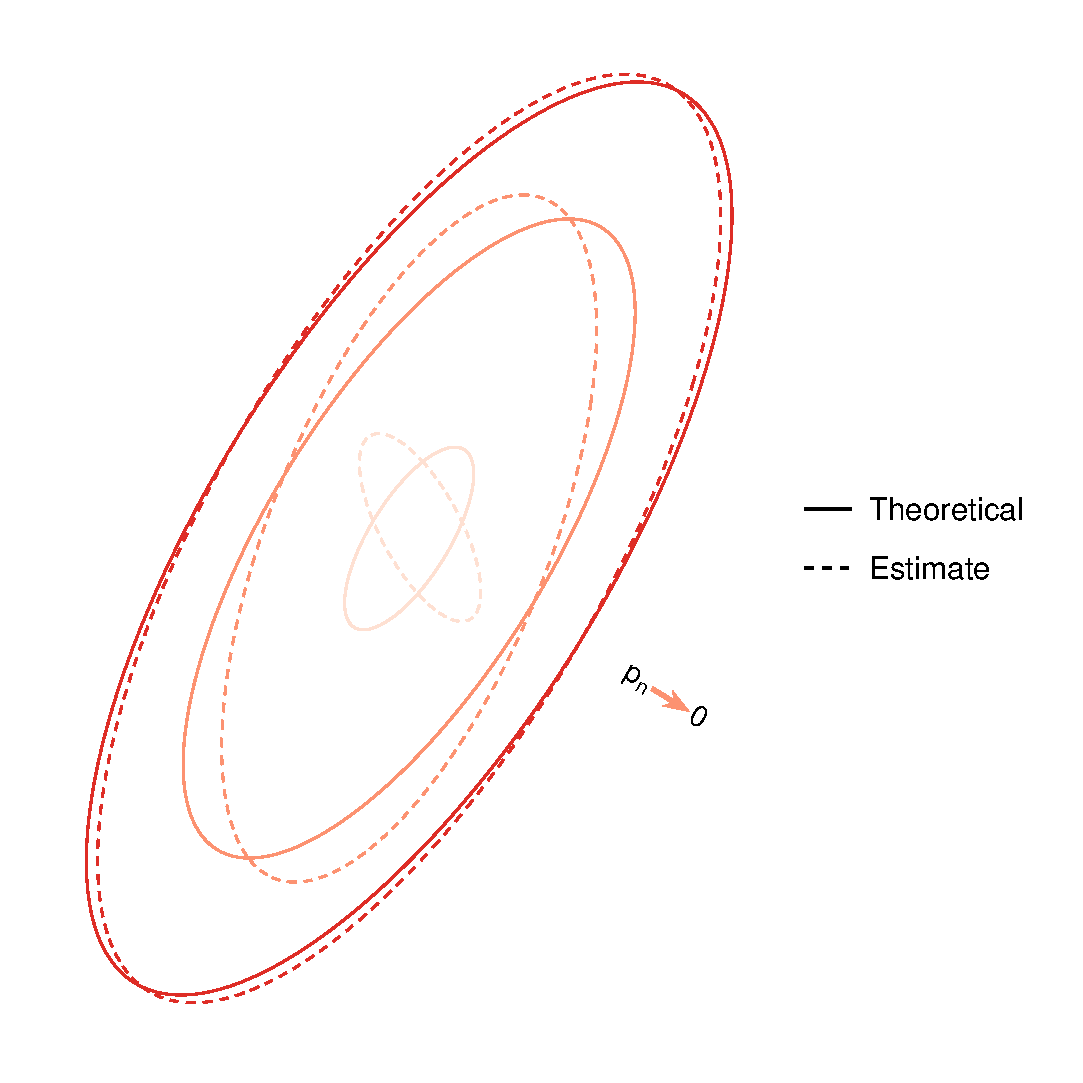
\includegraphics[width=0.8\textwidth, height=0.8\textwidth]{figures/consistency}
    \end{figure}
  \end{center}
\end{frame}

%%%%%%%%%%%%%%%%%%%%%%%%%%%%%%%%%%%

\begin{frame}
  Link to slides: \url{https://github.com/perej1/presentations/tree/main/light-error}
\end{frame}

%%%%%%%%%%%%%%%%%%%%%%%%%%%%%%%%%%%

\begin{frame}[allowframebreaks]{References}
  \printbibliography
\end{frame}
\end{document}
